

\pagebreak

\section{Background and Motivation}

E-learning providers are looking to improve the learning experience of their users and make progress as effective as possible. 
During a usual learning session each learner is subject to a range of volatile emotional states that help or hinder their learning success. 
A range of factors and stimuli, both internal and external, can influence emotions. 
When we take this knowledge about emotions into account a new way to manage a learning session opens. We can incorporate this knowledge into the learning sessions and provide a more appropriate task or interface for the learner.

The goal of the paper is to examine a relation between emotional aspect of a user interface in an e-learning system and its effect on performance of the learner.

\begin{figure}
	\begin{center}
		
\includegraphics[width=250px]{images/relation1.png}
		\caption{Relation Set 1\label{fig:relation1}}
	\end{center}
\end{figure}

\begin{center}
	
\includegraphics[width=200px]{images/relation1.png}
\end{center}
 
Several studies have shown correlation between emotion and cognition. In a similar fashion there is evidence of the surrounding environment having and strong influence on emotion \cite{Johnson2000, Arockiam2013, Bertamini2013}. This includes an e-learning system on the screen in front of the learner.

\begin{center}

\includegraphics[width=300px]{images/relation2.png}
\end{center}

Goal of the paper is to examine a relation between emotional aspect of a user interface in an e-learning system and its effect on performance of the learner.

There is a logical argument that a transitive relation between these parameters proves the dependency of the 2 edge variabled. 
Meaning exposure to several interfaces with different emotional charge during an online lesson should lead to a difference in performance on the same task.
Insufficient research confirming this connection and explaining the effects has been published yet. 
In this paper I would like to explore to which extent the final parameter can be influenced with the limited range of options that can tackle in a user interface on the screen.

\section{Approach and methods}

I propose a study that challenges human short-term memory, attention and creativity in a set of tasks. I will create a hypothetical learning environment that presents the same set of activities in 2 different interfaces, that should cause different emotions from the user. In a blind study each user would be given one of the interfaces and complete the tasks.

\pagebreak

\section{Approach and methods}

\subsection{Study Design}

I propose a study design that takes 4 groups of people, each group in one of the following states:

\begin{itemize}
	\item \textbf{Group1}: Positive valence / high arousal
	\item \textbf{Group2}: Negative valence / high arousal
	\item \textbf{Group3}: Positive valence / low arousal
	\item \textbf{Group4}: Negative valence / low arousal
\end{itemize}

Each test user would be preconditioned with help of audio-visual materials to be in one of 4 groups. 
Studies \citationneeded propose effective means to achieve this.

A short questionnaire (emotional awareness) will be used to validate, that preconditioning has had sufficient and expected effect on the subject.

A prepared task sequence (\ref{task_sequence}) will focus on testing short-term memory and creative/analytical problems. 
All groups would be presented with the same tasks but packed in 1 of 2 different interfaces.

50\% of each group would be presented with a task-set through Interface0 and 50\% would complete the tasks through Interface1.

\begin{itemize}
	\item \textbf{Inteface 0:} Default interface with low emotional capacity and standard language
	\item \textbf{Inteface 1:} Optimized interface with elements tailored for high arousal and positive valence emotion (potentially optimal for both memory and analytical tasks)
\end{itemize}

Both interface versions would provide equal usability features and should differentiate exclusively in emotional charge of its visual parameters.

After completing all tasks the subject will again answer the "emotional awareness" questionnaire to evaluate how their emotional state has changed to the previously recorded one, taken before the task

Effectively the study will build 8 groups of people (with both male and female subjects in each group).
It is my goal to have each testing sequence to be completed within 20 minutes time to keep the testing subjects' time investment low.
Statistical analysis will show whether differences in performance between groups could be observed. 

\begin{figure}
	\begin{center}
		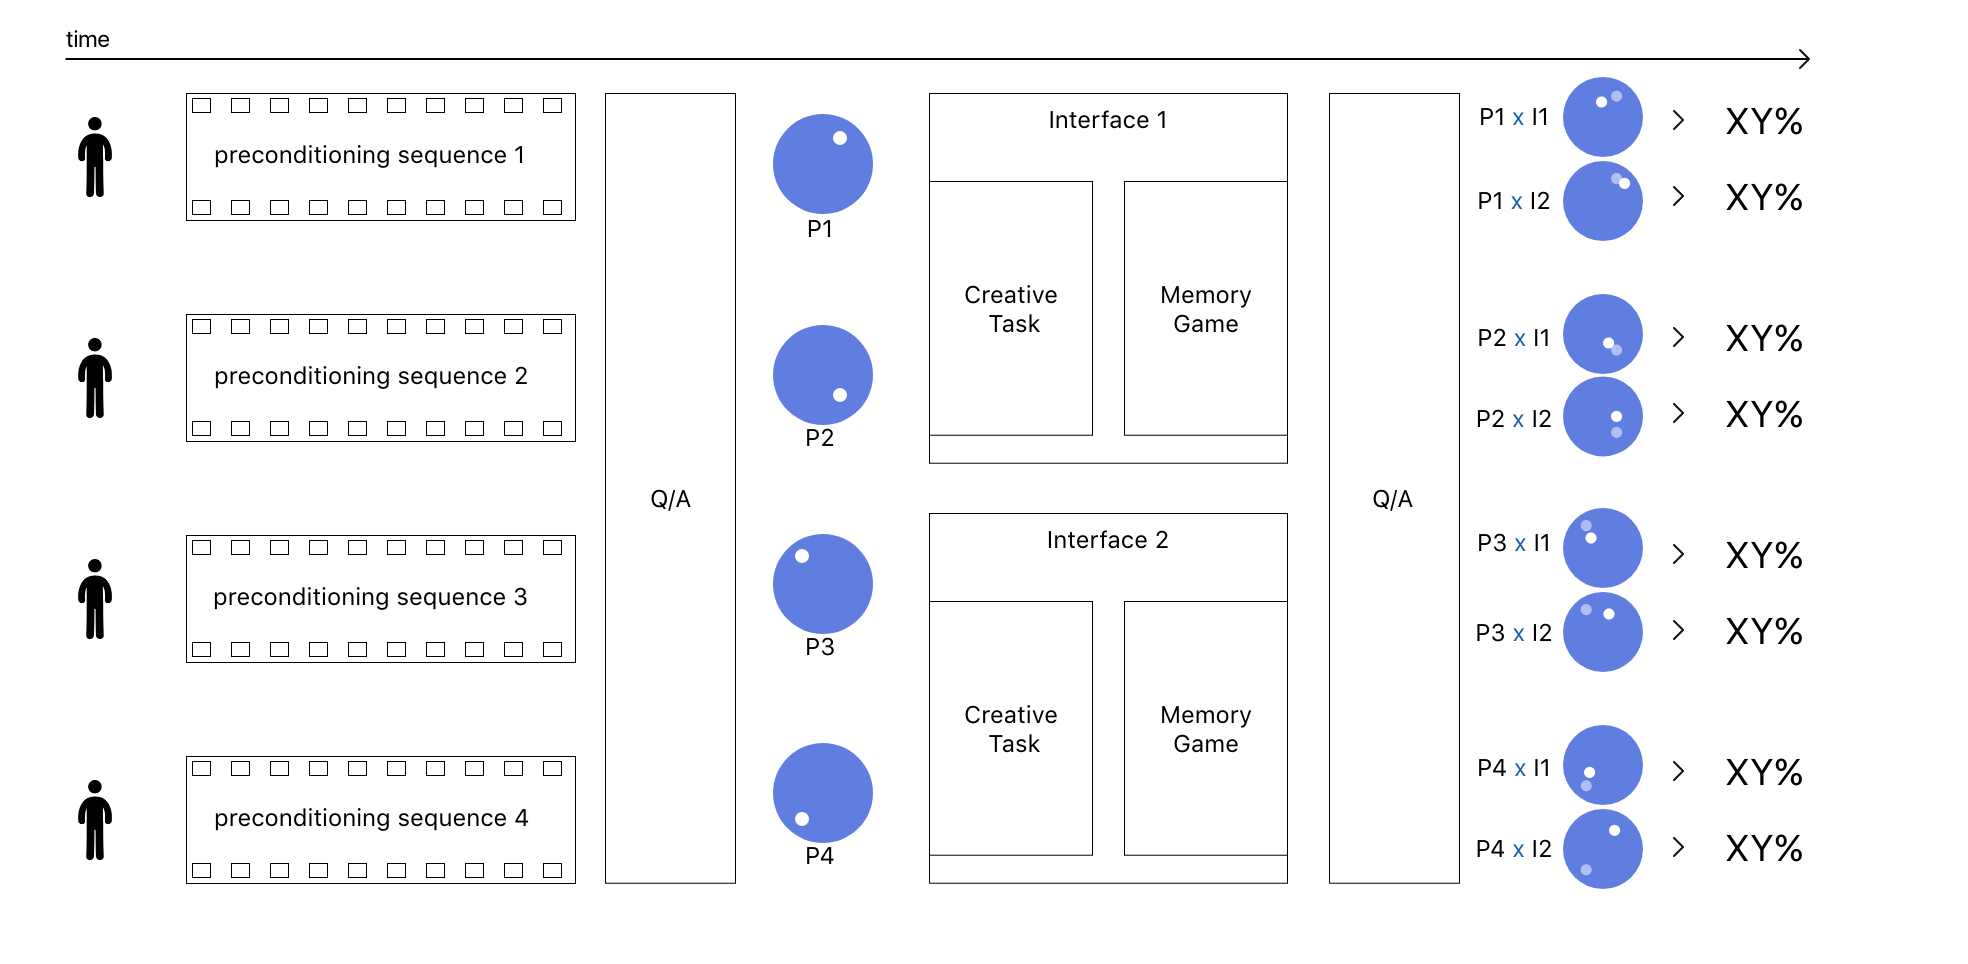
\includegraphics[width=1\textwidth]{images/study_design2.png}
		\caption{Study design\label{fig:scaled_diss}}
	\end{center}
\end{figure}

\subsection{Measuring performance} \label{measuring}

During each task several parameters will be recorded for each subject to create a comprehensive task performance metric. 
Examples include: rate of clicks per minute, mouse movements, rate of correct answers and time elapsed until completion can be measured. 

Mouse movement and video recordings could allow further qualitative analysis and provide room for more insight.

\subsection{Task Sequence} \label{task_sequence}

Psychological and cognitive studies have developed a variety of tests evaluating abilities of human mind. 
They differ in the art of activity and their focus, for example some concentrate on memory, creative thinking, analytical thinking, solving mathematical problems, imagination or orientation capabilities.

For this study I found several potentially fitting tests:

- \textbf{a classic memory game}. The goal is to find all pairs of images on a raster of (ex. 10 by 10) tiles. 
Only 2 pieces can be turned over at once. 
After which the turn back around and another try of finding a pair starts. 
The limitation of this game in the context of this study is that there is some degree of luck/chance involved in choosing correct tiles. 
To minimize it we could show all cards to the user for some seconds at the beginning of the game.
Expanding the field to more tiles would also reduce the chance influence in the beginning of the game, growing steadily towards the end.
It is possible to count only some amount of correct choices at the beginning of the game for evaluation and discard the ones that are turned over at the end of the game.
Another possible way to reduce chance behavior is to tag each tile if it has been turned over at least once. If it has then we could assume the player to have remembered the tile, otherwise count the tile choice as random chance choice and no count this move towards final evaluation of performance

- \textbf{Remote Associates Test}. Originally published by \cite[p.226 ff]{Mednick1962}, this test evaluates individual creativity. 
The test subject is presented with a set of 3 words and they must find a fourth word that is in some way connected to all three presented words.
This test is quite robust, yet for definitive results might require up to 40 minutes of testing time.

\subsection{Evaluation}

With quantitative analysis a more conclusive finding with significant results can be achieved with a larger amount of subjects participating in the study. 
Therefore the more I can get for this study - the better. 
I except that there will be at least 15 subjects per group (15 * 8 = 120 ) required.
To simplify acquisition of test subjects I will create a testing framework in the form of a web-application (See section \ref{implementation}), runnable on any browser.
With this uncontrolled approach to conducting the test there is a risk of noise within the testing environment (distractions and surrounding interference) and deliberately false answers skewing results.

\section{Implementation} \label{implementation}

To facilitate the study I will build a web application (based on reactjs), runnable on desktop and tablet devices. Data emitted from the application will be saved in a remote database (mongodb) for the purposes of evaluation.

Every subject would be presented with one of 4 preconditioning sequences and one of 2 interfaces on a semi-random basis.

No information should be stored locally on the device after finishing a session.

\section{Implications of the study}

If this study can demonstrate a significant difference in performance across groups, we can conclude that emotional features of digital user interface can have a noticeable impact on the way people consume information, memorize and analyze problems.
It will pave the way for further studies being done exactly which aspects of an interface have the biggest impact and how to design for sustained attention and performance.

E-learning providers can use these findings to better structure their online lessons and invest in design that supports the learner.

Further these findings can be adapted and generalized to make use of within other applications in software, digital media and similar outlets.

\section{Ethical, legal and social considerations}

Conducting this research will require several subjects' actions to be recorded and stored for evaluation purposes.
Anonymized, semi-personal (gender, age) as well as some sensitive information (video recording, with users consent) could be transferred to a server and saved for the duration of the study.
After the study, all sensitive and personally identifiable data will be removed and aggregated to facilitate anonymity.